\setstretch{1.6}
\sectiontitle{6}{Software Refactoring}
\lhead{Software Refactoring} % section header

\subsection{Theory}
\subsubsection{Software architecture for real-time systems}
Real-time systems require software that is predictable and responsive, even under strict timing constraints. This places additional demands on the software design, especially since codebases for such system may grow rapidly when there is necessity for GUI handling, hardware commands, control calculations and communication protocols. According to McConnel \cite{steve_mcconnell_code_nodate}, high-quality architecture in such systems should emphasize simplicity, clarity, and robustness to change. 
\newline \newline
A well-structured architecture improves maintainability and extensibility by making the system easier to understand and reason about. In real-time contexts, this often translates into an architecture that minimizes dependencies betwen components and provides clear seperation between hardware interaction, control logic, and application-level coordination \cite{tanenbaum_distributed_2007}.

\subsubsection{Modular design principles}
Modularity is one of the most important design principles when managing software complexity. Modular systems break down functionality into discrete units that encapsulate behavior and expose minimal interfaces \cite{steve_mcconnell_code_nodate}. This separation reduces the mental burden on developers and allows individual parts of the system to be developed, tested, and modified independently—greatly improving maintainability and scalability.
\newline \newline
Effective modularity hinges on two key design goals: low coupling and high cohesion. Low coupling refers to moules having minimal dependencies on each other, and high cohesion means that all parts fo a module contribute to a single, clear purpose \cite{steve_mcconnell_code_nodate}. These ideas build on the concept of "information hiding" \cite{parnas_criteria_1972} where internal implementation details are kept private, preventing unintended interactions across modules.

\subsubsection{Threading and concurrency}
Concurrency is often necessary in real-time systems to meet iming constraints and maintain responsiveness. Use of threads allows the system to perform multiple tasks concurrently, such as sensor data acquisition, visualization, control loop comuptation and user interaction, without blocking the main execution path.
\newline \newline
However, introducing concurrency also introduces complexity. Issues such as race conditions, deadlocks and nondeterministic behavior must be managed. McConnell \cite{mcconnell_code_2004} warns that improperly designed concurrency can reduce the reliability of software rather than improve performance. Therefore, concurrent systems should be built using clear a clear design, thead-safe communication mechanisms and minimal shared states \cite{noauthor_software_nodate}.

\subsubsection{Event-driven communication in Qt}
A common and reliable pattern for concurrent real-time systems is event-driven communication between threads. In this model, components communicate through asynchronous messages rather than direct calls or shared varieables. In Qt this is implemented via the signal-slot mechanism. Signals are emitted when events occur, and slots (connected handler functions) respond to those events. Qt ensures that the communication is thread safe by searializing signal delivery using the vent loop of the receiving thread, meaning that it will execute in the context of the receiving threads event loop. 

\subsection{Methods}
\begin{wrapfigure}{r}{0.55\textwidth}
    \centering
    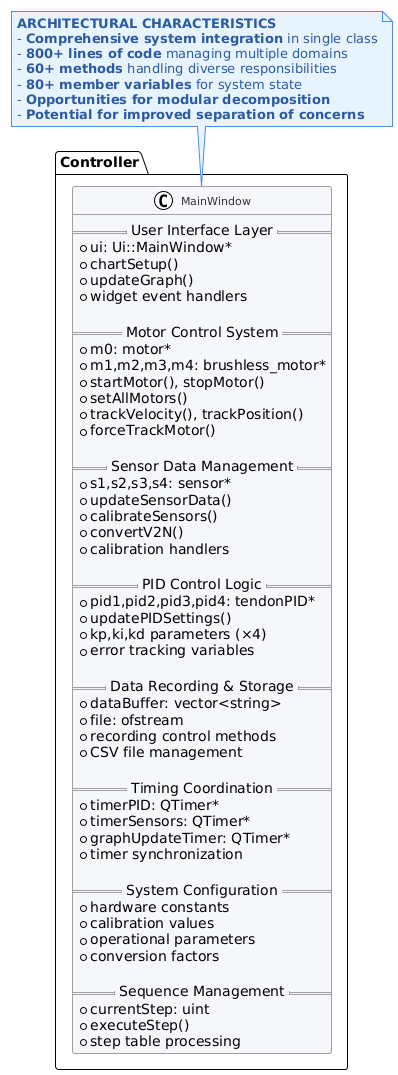
\includegraphics[width=\linewidth]{images/Software documentation/old code/mainwindow2.png}
    \caption{Original Mainwindow implementation, prior to refactoring}
    \label{fig:oldmainwindow}
\end{wrapfigure}
The refactoring process began with a thorough analysis of the existing codebase. Throughtout this process the existing methods and classes were documented using a style compatible with doxygen. This step provided an overview of the software architecture and highlighted areas where the structure violated modular design principles, such as excessive coupling and low cohesion.
\newline \newline
An analysis of the original codebase showed that there were several issues especially low cohesion and a large range of responsibilities in the mainwindow class, leading to low readability as is exemplified in figure ...
\newline \newline
The original architecture senn in \ref{fig:oldarchitecture} made sense for the application with classes for the motors, the tendon pids etc, but since some responsibilites that should have belonged to those classes remained in the mainwindow the architecture wasn't very useful and the code had high interdependence and very little abstraction.
\begin{figure}
    \centering
    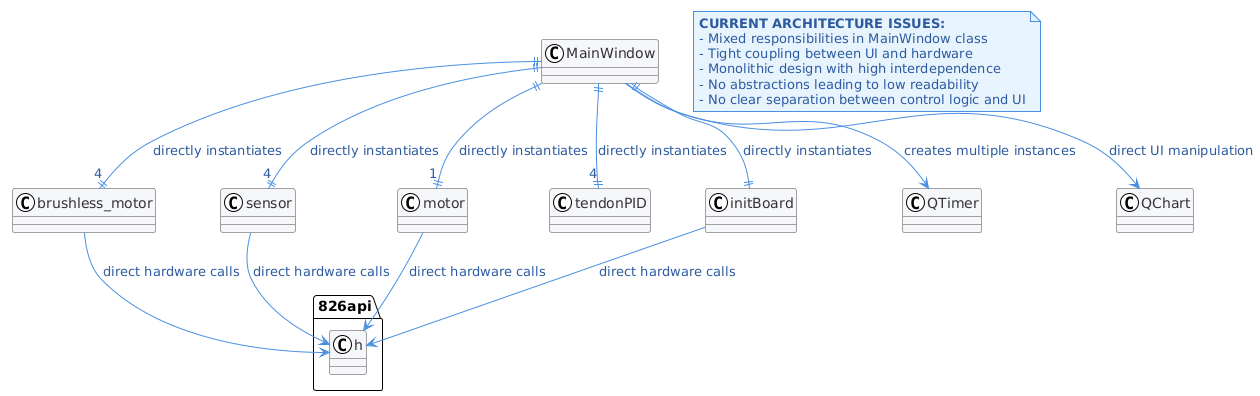
\includegraphics[width=1.15\linewidth]{images/Software documentation/old code/architecture2.png}
    \caption{Original architecture, prior to refactoring}
    \label{fig:oldarchitecture}
\end{figure}
Based on the architectural guidelines described in the theory section, a revised design was developed. The design emphasizes smaller highly cohesive classes and separation of concerns by defining minimal, well-documented interfaces between modules and isolating hardware-dependent functionality, for different types of application level logic. The existing code was refactored to fit into this structure and unnecessary functionality was removed. Existing errors in the code were also remedied. Thereafter new code was written into the the modules in order to expand the functinality of the system.

\subsection{Implementation}
Before the refactoring process, much of the application logic was concentrated in \texttt{mainwindow.cpp}. It was restructured into well defined modules, each responsible for a specific task. The updated project structure includes:
\begin{itemize}
    \item \textbf{motorcontrol/}: Manages low-level motor and linear stage control.
    \item \textbf{pathfollowing/}: Handles trajectory processing, feedforward calculations, and path interpolation.
    \item \textbf{tendonpids/}: Contains the PID control logic for tendon tension regulation.
    \item \textbf{vision/}: Manages communication with external vision systems.
    \item \textbf{Core files (e.g., \texttt{main.cpp}, \texttt{mainwindow.cpp})}: Responsible for application startup and GUI logic.
\end{itemize}

The entire system follows and event-driven architecture using Qt's signal-slot mechanisms wherever possible. This reduces the need for extensive multithreading as modules do not block threads for long periods. Instead most classes react to signals or timers. Some components, such as sensor data acquistion and closed-loop tension control, operate on fixed update intervals using timers. Others, like the path-following controller are triggered by receiving a new vision measurement.
\newline \newline
To support real-time perfomance and responsiveness, multithreading was introduced where strictly necessary. Only components that demonstrated clear performance bottlenexs or responsiveness issues were moved to separate threads. The following components run in dedicated threads:
\begin{itemize}
    \item \textbf{Logging thread}: Records sensor and control data without blocking the main loop.
    \item \textbf{Motion estimation thread}: Continuously estimates stage speed at a high frequency while the linear stage is running for use in feedforward for the closed loop tension control.
    \item \textbf{Vision receiver thread}: Continuously listens for incoming vision data and receives and parses it.
\end{itemize}


\subsection{Results}

\begin{figure}
	\centering
	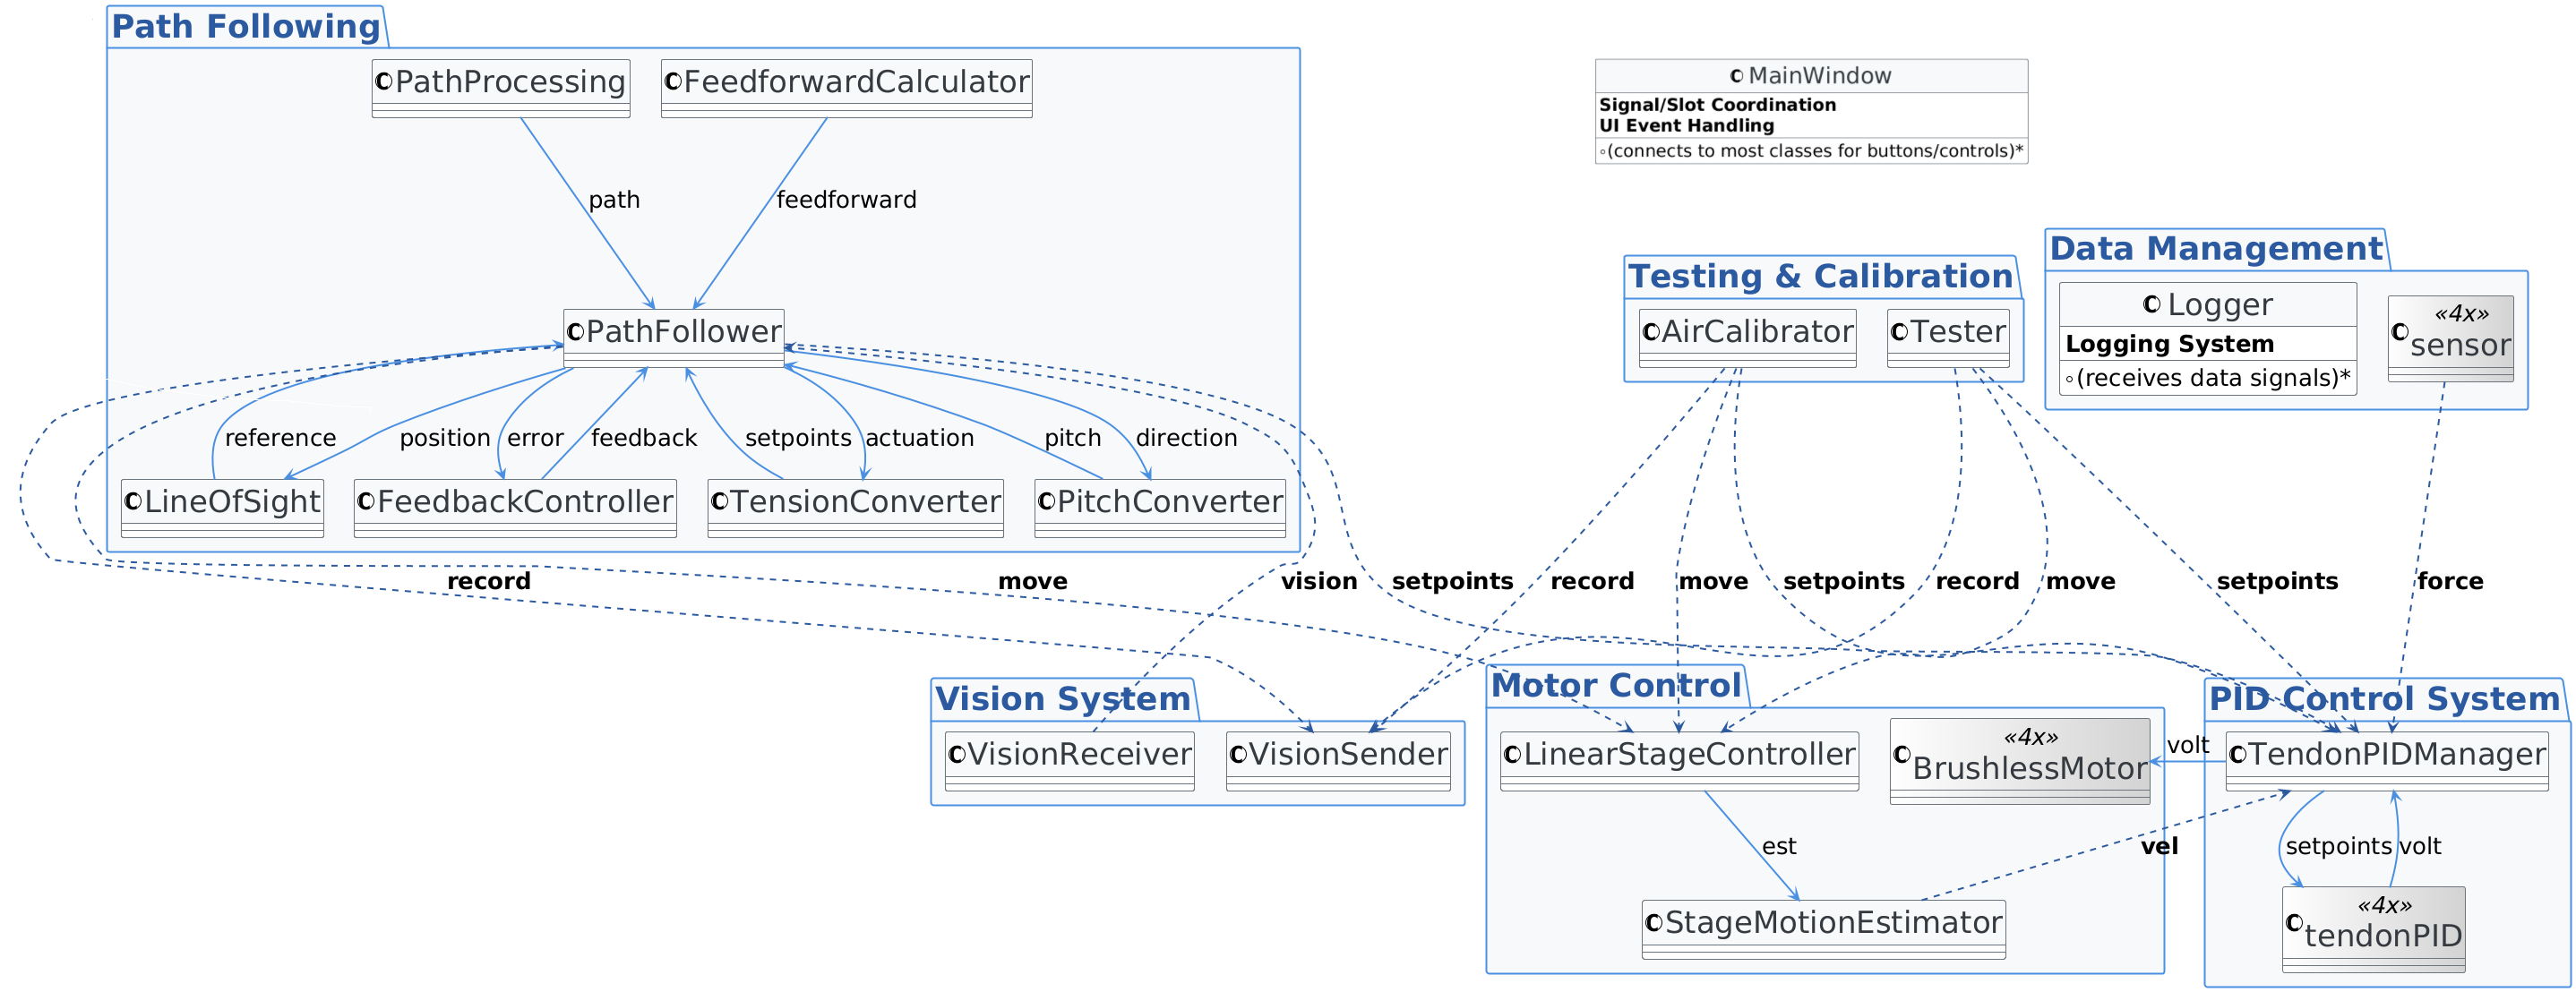
\includegraphics[width=\linewidth]{images/Software documentation/architecture3.png}
	\caption{Final control code base architecture after refactoring}
	\label{fig:architecture}
\end{figure}



\todo{figure of new architecture!}
\todo{figure of threads!}



\subsubsection{Sensor}
The \texttt{sensor} class was restructured to encapsulate all low-level configuration and data handling required for each individual sensor. Upon initialization, it configures the ADC to sample at the correct timeslot, sets the analog input gain, and synchronizes data acquisition with a dedicated counter using external trigger modes. This ensures that each sensor samples consistently and at the intended \SI{1}{\kilo\hertz} rate. The class also handles voltage-to-force conversion using sensor-specific calibration constants, allowing for flexible reuse across different sensors with varying sensitivities. The readout function returns both the converted voltage and the corresponding timestamp, ensuring the measurements are correctly time-aligned with the control loop. By modularizing the sensor interface in this way, the implementation became more maintainable, reusable, and easier to debug during both development and calibration.

\subsubsection{PI controller}
The feedback controller runs on a timer loop synchronized with the sensor update rate. It is structured to remain modular and extendable, with clearly defined interfaces for input (force readings and setpoints) and output (motor commands), enabling easy replacement or augmentation with more advanced controllers (e.g., adaptive or model-based) in future work.

\subsection{Discussion}


By combining lightweight threads for parallel execution with queued, thread-safe communication via Qt signals/slots, real-time systems can achieve both responsiveness and reliability without falling prey to classic concurrency pitfalls.

Only components that demonstrated clear performance bottlenecks or responsiveness issues were moved to separate threads. This approach minimizes complexity while still meeting the system’s real-time requirements. Communication between modules is kept minimal and modular, consistent with the design principles of low coupling, high cohesion, and information hiding discussed in the theory section.

The result is a system that is easier to maintain, extend, and test, with clear module boundaries and a simplified control flow.

By relying on Qt’s signal-slot mechanism, the system maintains responsive behavior while keeping communication between modules clean, thread-safe, and loosely coupled.

This approach allows the system to meet its real-time requirements while maintaining simplicity and modularity in both structure and execution flow.




